\documentclass[12pt]{article}
\usepackage[utf8]{inputenc}
\usepackage{fullpage}
\usepackage{graphicx}
\usepackage{url}
\usepackage{amsmath}
\usepackage{amssymb}
\usepackage{caption}
\usepackage{subcaption}
\usepackage{color,soul}
\usepackage{amsfonts}
\usepackage{wrapfig}
\usepackage{multicol}
\usepackage{hyperref}
\hypersetup{
   colorlinks=true,
   linkcolor=blue,
   filecolor=magenta,
   urlcolor=cyan,
   pdftitle={laboratory02–AISC},
   pdfpagemode=FullScreen
}
\graphicspath{ {./images/} }
\usepackage{fancyhdr}
\usepackage{enumitem}
\usepackage{epigraph}
\setlist[itemize]{noitemsep, topsep=0pt}
\setlist[enumerate]{noitemsep, topsep=0pt}
\title{Laboratory 2 – AISC}
\author{Agnetta Stefano, Brozzo Doda Umberto, Macario Davide}
\date{March 29\textsuperscript{th}, 2023}

\newcommand\titleofdoc{Laboratory 2 – AISC} %%%%% Title
\newcommand\GroupName{Agnetta Stefano, Brozzo Doda Umberto, Macario Davide}
\newcommand\CurrDate{March 29\textsuperscript{th}, 2023}

\begin{document}
\begin{titlepage}
   \begin{center}
        \vspace*{4cm} % Adjust spacings to ensure the title page is generally filled with text

        \Huge{\titleofdoc} 

        \vspace{0.5cm}
        \LARGE{A simplified version of AES}
            
        \vspace{3 cm}
        \Large{\GroupName\\}
       
        \vspace{4 cm}
       
        \vspace{4 cm}
        \Large{\CurrDate}
        
        \vspace{0.25 cm}
        \Large{A.Y. 2021–2022}
       
       \vfill
    \end{center}
\end{titlepage}

\section{Introduction}
\label{sec:01}

This laboratory revolved around the analysis of a simplified version of AES (Advanced Encryption Standard), which was provided as a python script, which can be found at~\cite{Original Python implementation}, and which also contained all necessary sub–blocks for each round (SBox, ShiftRows, MixColumns and AddKey).

These blocks are designed to work on 16–bit inputs, organized as 2–by–2 matrices of 4–bit `\textit{nibbles}'. Also the key is a 16-bit string.

The focus of this analysis is to test the behavior of the simplified AES in terms of avalanche effect, and to cryptanalyze an improper implementation of a block cipher, based on the provided sub-blocks, in order to break a ciphertext.

\section{Avalanche effect}
\label{sec:02}

The goal of the first section of this laboratory was to demonstrate the avalanche effect of the simplified AES that follows a single bit flip after various manipulations of the algorithm, such as different number of rounds and the missing implementations of some fundamental steps.

To measure the avalanche effect the hamming distance will be computed: values around half the length of the elements in exam mean a good avalanche effect, since the correlation between them is at its lowest point.

Two different experiments will be taken.
In the first one, given a key, a plaintext is randomly generated and encrypted, then a bit of the plaintext is flipped and the result is encrypted. The key used is: \verb|0b1111111111111111|.
In the second one, chosen a plaintext, the key is randomly generated and used to encrypt the plaintext; the same plaintext is then encrypted with the key with a single bit flipped. The used plaintext is: \verb|0b1010101010101010|.
Both the experiments are repeated 1000 times, and the avalanche effect is measured referring to the average of the hamming distances of each single run.

Since they will be recalled more times, for the sake of convenience they will be respectively called ``changed plaintext'' and ``changed key'' experiments.

In the first step, the algorithm is composed of all its four fundamental blocks, which will be repeated two times. For the ``changed plaintext'' experiment the average hamming measured is around \verb|4|, and a value of \verb|8| is obtained for the ``changed key''.
The resulted diffusion property of the ``changed key'' is explained by the fact that when, during the second round, the key expansion is performed it changes radically the key itself, so the new state (obtained evaluating the XOR between the key and the current state) will statistically become completely different from its starting value.
The other first experiment shows instead a weaker behavior: the state is treated as four blocks, and a change in one of them does not necessarily result in big differences after just two rounds of AES\@. Indeed, as the the number of rounds raises to 3, the avalanche effect measured starts to converge to values around \verb|8| for both the experiments.
As the number of rounds raises the results continue to show a good average hamming distance, which sets to 3 the number of minimum rounds needed to have a sufficient avalanche effect.

Now, for the next following step, referred to as ``lazy version'', ShiftRows and MixColumns blocks are missing and as the experiments are done, the hamming distances decrease drastically for the ``changed plaintext'' experiment. This enlights how the diffusion property is strongly dependent on ShiftRows and MixColumns blocks. The reason lies in the way these two stages operate: they provide bit shuffling between different 4-bits nibbles of the state, and consequently, if these stages are skipped, the difference between two ciphertexts obtained from two plaintexts which have hamming distance equals to \verb|1| cannot be more than 4, which is the size of a nibble.

\begin{table}[h!]
    \centering
    \scalebox{0.65}{
    \begin{tabular}{|r||l|l|}
    \hline
        & Plaintext & Ciphertext\\
        \hline
        \hline
        Instance 1 & 1010 1010 1010 1010 & 0111 0001 0001 0011\\
        \hline
        Changed values for instance 1 & 1010 1110 1010 1010 & 0111 0010 0001 0011\\
        \hline
        \hline
        Instance 2 & 0010 1010 0110 1110 & 1111 1011 1100 0101\\
        \hline
        Changed values for instance 2 & 0010 1011 0110 1110 & 1111 0100 1100 0101\\
        \hline
    \end{tabular}}
    \caption{Two results (in blocks) of the "changed plaintext" experiment ("lazy version")}
\end{table}

In any case, this ``lazy version'' still produces an appreciable diffusion effect for the ``changed key'' experiment after a slight change in the key.

The last test, called ``very lazy version'', follows a cut on the key expansion block's behavior, so that only the first two round keys will be used for all the rounds. Finally the encryption becomes now ineffective, giving hamming distance values around \verb|2| for both the experiments. Now a single bit change to the key in the ``changed key'' experiment will end in a less diffused result, since only the first two subkeys obtained from the key expansion (which values correspond to the first and the second byte of the key respectively) are used for the encryption.

These experiments showed how the AES algorithm needs to be fully implemented to grant diffusion and confusion properties in every cases, so that cryptanalysis techniques are almost impossible to be performed.

\begin{table}[h!]
    \centering
    \scalebox{0.65}{
    \begin{tabular}{|c||l|l|l|l|l|}
    \hline
        & 2 rounds & 3 rounds & 4 rounds & 4 rounds, lazy implementation & 4 rounds, very lazy implementation\\
        \hline
        \hline
        flipping one bit in the plaintext & 4.229 & 8.646 & 7.987 & 2.107 & 2.108 \\
        \hline
        flipping one in the key & 8.053 & 8.041 & 7.881 & 7.998 & 2.055\\
        \hline
    \end{tabular}}
    \caption{Average hamming distance between ciphetexts}
\end{table}


\section{Improperly implemented block cipher}
\label{sec:03}

The second part of this laboratory concerned the cryptanalysis of an improperly-implemented block cipher whose implementation was given, and which used on the blocks that were provided for the simplified AES.\@

The task was essentially that of carrying out a KPA having observed a single plaintext-ciphertext pair, which was obtained with the same key as another large ciphertext that needed to be broken.
The pair was the following:

\begin{itemize}
   \item \textbf{Known plaintext}: \verb|0b0111001001101110|
   \item \textbf{Known ciphertext}: \verb|0b0001111001100101| 
\end{itemize}

Having the possibility to observe the Python code which implemented the encryption (and decryption) mechanism, it was found that the block cipher consisted of a single round, composed of ``Substitute Bytes'', ``Shift Rows'' and ``Add Key'' (with a 16-bit subkey) blocks only, whose order was reversed for decryption.
This structure already highlights one main security issue, as the lack of an initial ``Add Key'' stage makes it so that the knowledge about the bits before the last ``Add Key'' automatically reveals the plaintext (the remaining stages do not contain `secrets' such as the key).

Furthermore, the key expansion procedure proposed for the simple AES can be seen to produce as subkeys $k_0$ and $k_1$ the first 8 bits and the last 8 bits of the original key, respectively. For this reason, the key which is added during the last (and only) ``Add Key'' stage corresponds to the actual key itself, as provided by the user.

Figure~\ref{fig:3.1} shows the structure of the described block cipher.

\begin{figure} [ht]
   \centering
   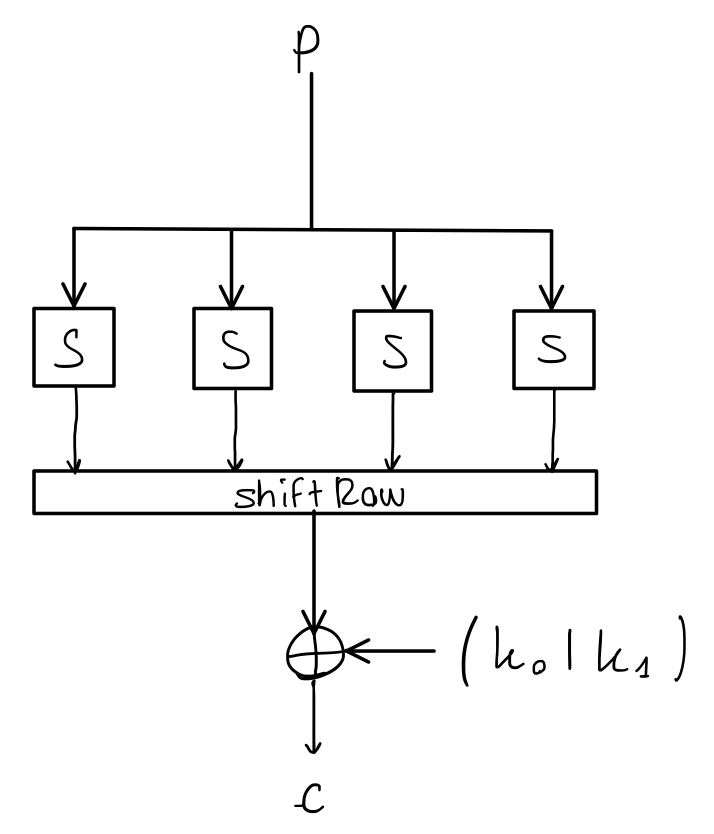
\includegraphics[width = .5\linewidth]{improper_block_scheme.jpeg}
   \caption{Structure of the improperly implemented block cipher}
   \label{fig:3.1}
\end{figure}

Putting all these things together, the proposed (known plaintext) attack consists in performing the first two stages on the known plaintext (``Substitute Bytes'' and ``Shift Rows'') and then directly finding the key by evaluating the XOR between the result of the first stages and the known ciphertext. This last step guarantees the discovery of the key (in theory the ensemble of sub-keys $k_0$ and $k_1$), thanks to the properties of the XOR operator ($A\oplus B = C\ \implies A\oplus C = B$).

By performing these steps, the key used in the known pleintext-ciphertext pair was found to be \verb|0b100000111101111|.

The ciphertext was then decrypted, knowing the block cipher was used on two characters at a time (16 bits total).

The resulting plaintext contained a quote from `The Lord of the Rings':

\begin{quote}
   \textit{When Mr.\ Bilbo Baggins of Bag End announced that he would shortly be celebrating his eleventy-first birthday with a party of special magnificence, there was much talk and excitement in Hobbiton. 
   Bilbo was very rich and very peculiar, and had been the wonder of the Shire for sixty years, ever since his remarkable disappearance and unexpected return. 
   The riches he had brought back from his travels had now become a local legend, and it was popularly believed, whatever the old folk might say, that the Hill at Bag End was full of tunnels stuffed with treasure. 
   And if that was not enough for fame, there was also his prolonged vigour to marvel at. Time wore on, but it seemed to have little effect on Mr.\ Baggins.
   At ninety he was much the same as at fifty. 
   At ninety-nine they began to call him well-preserved, but unchanged would have been nearer the mark. 
   There were some that shook their heads and thought this was too much of a good thing; it seemed unfair that anyone should possess (apparently) perpetual youth as well as (reputedly) inexhaustible wealth}
\end{quote}

\subsection{Decryption under COA}
\label{sec:03.1}

As seen, breaking the encryption scheme under KPA is simple, as the mechanism lacks the initial XOR operation between plaintext and sub-key.
Supposing there is no available known plaintext–ciphertext pairs, the approach taken by an attacker needs to be different.

The overall encryption process for a long plaintext (such as the one in `ciphertext.txt'), then becomes similar to that of a Vigenère cipher, in which different portions (blocks) of the message are encrypted in the same way. In particular, after being passed through the S-Boxes and the ``Shift Rows'', the same key is applied on every set of 2 characters (16 bits).

The presence of the two initial sections, however, makes it difficult for the opponent to proceed in the same way as in laboratory 1, i.e., by performing frequency analysis of the (two) subsequences. Indeed, thanks to the confusion introduced by the `Substitute Bytes' and `Shift Rows' blocks, which cause bits from the first of the 2 characters to have an impact on the last 8 bits, and vice–versa.
As a result, each character in the ciphertext essentially depends on two characters from the plaintext.
This makes it impossible to cryptanalyze this block cipher in the case of a Ciphertext Only Attack and for this reason the only viable attack is to brute force the 16-bit key.
The only approach that may be followed to slightly simplify the search could be that of realizing that the same couple of (ordered) characters are associated to the same couples of characters in the ciphertext, since, even if improperly implemented, this block cipher has been defined to be invertible.


\section{Conclusions}
\label{sec:04}

During this laboratory experience it was possible to experiment with a trivial implementation of AES, which helped in getting some insights on how actual AES implementations behave.

It was interesting to really see how the algorithm is able to achieve the avalanche effect and how it this is important in guaranteeing an effective encryption.

The study of the improperly-implemented block-cipher-based encryption mechanism, instead, provided a way to analyze block ciphers from the security point of view, by effectively highlighting the possible attack surfaces of poorly implemented solutions.

\begin{thebibliography}{5}
   \bibitem{Original Python implementation} \url{https://jhafranco.com/2012/02/11/simplified-aes-implementation-in-python}
\end{thebibliography}

\end{document}